% Chapter 4 - Description of Nek

\chapter{Application of Nek5000} % Main chapter title

\label{nek} % Change X to a consecutive number; for referencing this chapter elsewhere, use \ref{ChapterX}

\lhead{Chapter 4. \emph{application of Nek}} % Change X to a consecutive number; this is for the header on each page - perhaps a shortened title

%----------------------------------------------------------------------------------------
%	SECTION 1
%----------------------------------------------------------------------------------------


%\colorbox{green}{ta med flyttdiagram for l;sningen}
%\colorbox{green}{rydd opp i skjemaene! referer til en l;rerbok, beskriv vha numerisk flow phi\ldots }
%\colorbox{green}{Hver tydelig paa hva man itererer over.}
%\colorbox{green}{korte ned tekstene!}
There are many numerical solvers for turbulent flows available on the market.
From large commercial softwares such as Fluent which runs as a 
black-box solver, to full open-source codes such as Nek5000 and openFOAM. 
The solvers can vary in the numerical method; Finite volume, Finite Differences, 
Finite Element Method, Spectral Element Method etc., The particular algorithm 
for resolving the Pressure-Velocity coupling, for instance Fractional Step, Poisson pressure and 
Uzawa. The type of simulation available also varies from solver to solver, whether
they apply RANS, LES, DNS or a variety of these. Although most solvers offer multiple of the settings
listed above it is important to be aware of their strengths and weaknesses before choosing which 
one to use. This section will be devoted to the handling of Nek5000, and can serve
as a brief introduction to the code.

\section{Nek5000 basics}

Nek5000 is a turbulent flow solver developed mainly by Paul Fischer
and has through the past 20 years had several contributors. 
It is an open-source code applicable to many different types of flow 
and it has been put a lot of effort into the parallelization of the code, 
guaranteeing optimal speedup. All the parallelization is accessed through subroutines
and functions, enabling the user to make advanced functions without having to 
deal directly with the functions from the MPI library.
With SEM as the numerical method applied it is possible to obtain very accurate results.  

%nek5000 has its own mesh-generator for generating simpler geometries and it is also implemented the possibility to integrate CUBIT mesh 
%files. A common starting point for simulating turbulent flow is a geometry given by a CAD-file,
%without any functions to describe the boundaries.
%The possibility to make a mesh through a visual gui is provided through for instance ICEM.
%This mesh can then later be transformed to the inputfile required by Nek5000. 

Nek5000 provides some basic tools for generation of mesh. For more complex geometries this tool cannot compare with more visualized-based softwares 
such as ICEM from ANSYS which exports mesh to several numerical solvers such as Fluent and Nastran.
It is therefore very useful to have an automatic way of converting a mesh created in ICEM to the format required by Nek5000. 
The way the mesh is created in this thesis is visualized in \fref{fig:mesh}.
%
\begin{figure}[h]
	\centering
	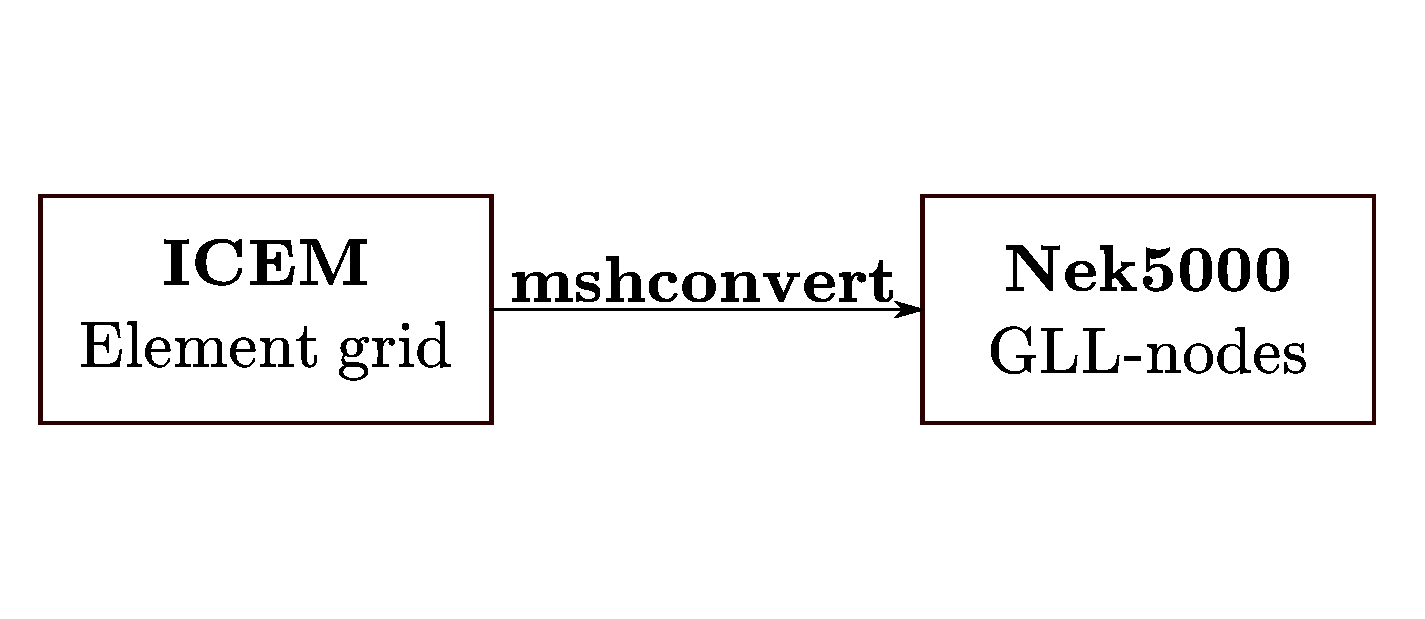
\includegraphics[width=0.6\textwidth]{Figures/mesh.pdf}
	\caption{Visualization of how the mesh is created. The elemental mesh is first generated using ICEM, the script mshconvert
    converts this to a .rea-file and finally the distribution of the GLL-nodes is done during the initialization in Nek5000}
	\label{fig:mesh}
\end{figure}
%
%In order for Nek5000 to run optimally the elements should be as homogenous and as similar to the reference element as possible. 
%It is therefore of great interest to be able to propagate curved geometries into the neighbour-elements in order to have a smooth as 
%possible transition from a boundary with high curvature.

So far Nek5000 has supported three automatic routines for generating curved edges;
circles in 2-D geometries, spherical shell elements and a general 2nd degree interpolation.
Further manipulation of the element edges is left to the user to define manually
for each particular problem. One of the objectives of this thesis is to make Nek5000 more
user-friendly and create automatic routines to handle complex geometry. Before the work regarding
the mesh routines are further elaborated an overview of the file-structure will be presented.

\section{Editable files}
%
\begin{figure}[h]
	\centering
	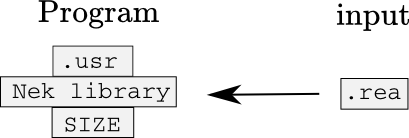
\includegraphics[width=0.5\textwidth]{Figures/filestructure2.png}
	\caption{Visualization of how the file structure in Nek5000 is built up.}
	\label{fig:files}
\end{figure}
%
In order to work with Nek5000 there are some practical information that needs to be clarified.
Nek5000 is recompiled for every case and the user specify all the case specific 
information in the three files \verb|{.rea,.usr,SIZE,}|. \verb|.usr| and \verb|SIZE| are 
compiled with the standard Nek5000 library using makenek which creates the executable file \verb|nek5000|,
they can be considered the surface and the core of the entire program. 
The \verb|.rea| file contains case-specific information read during the initialization of the 
compiled program. The user guide \cite{Nek} contains a tutorial which explains the necessary 
steps on how to get started with Nek5000. The next chapters will try to give some understanding on 
how the user is able to make the changes necessary for each case. \fref{fig:files} illustrates 
how the files work together. 
%
\subsection{SIZE}
Since Nek5000 is mostly based on Fortran77 all memory allocations are done statically and must be specified explicitly 
before runtime. Most of the variables used to determine the memory usage are stated in \verb|SIZE|.
The size of the working arrays necessary to perform the calculations are mostly defined by the upper limits of elements, 
processors, scalars and of course the polynomial degree
of the local Lagrange functions. These variables define the sizes of almost all 
the arrays used in the program so it is important to define these variables as accurately 
as possible in order to optimize memory usage. The \verb|SIZE| file can be considered as the necessary base 
for Nek5000.
%\begingroup
%\fontsize{12pt}{14pt}
%\begin{lstlisting}[escapechar=|,frame=none]
%parameter (ldim=3)                                   ! dimension
%parameter (lx1=6,ly1=lx1,lz1=lx1,lelt=600,lelv=lelt) ! GLL-points,elements/processor
%parameter (lxd=9,lyd=lxd,lzd=lxd)                    ! Order of De-aliasing
%\end{lstlisting}
%\endgroup
\subsection{.rea}

In \verb|.rea| all the problem specific parameters are given. While the content in \verb|SIZE| 
is an absolute necessity to even compile the program the \verb|.rea| file contains variables 
that are not used until the initialization of the case. The structure of the file is given in \tref{tab:reafile}.
Of the 103 variables specified in the beginning of the file there are roughly 50 of them that are used. 
Note that apart from the mesh information the \verb|.rea| file restricts itself to single variables and boolean flags 
while the \verb|.usr| needs to be applied for more advanced implementations. 
%
\begin{table}[h]
    \centering
    \begin{tabular}{c c l}
       Lines & Section Name & Specifications \\ \hline
       $103$ & PARAMETERS & All problem-specific variables \\ 
       $K$ & PASSIVE SCALAR DATA & Convective and diffusive constants for scalars\\ 
       $K$ & LOGICAL SWITCHES & Boolean variables defining the solution method \\ 
       $E$ & MESH DATA & All nodes and elements are specified here\\
       $E$ & CURVED SIDE DATA & All the curved sides are specified here\\
       $E$ & FLUID BC& BC type for all elements and their faces\\
       $E$ & THERMAL BC& Thermal BC type for all elements and their faces\\
       $K$ & PRESOLVE/RESTART & Filename(s) of an initialized solution \\
       $K$ & INITIAL CONDITIONS & possibilities to specify IC further \\
       $K$ & OUTPUT FIELD & information that will be written to file\\
    \end{tabular}
    \caption{An overview of the different sections in .rea. $E$ represents a predefined number depending on your problem
    which scales roughly as the number of elements, while $K\approx 1-25$ are user defined numbers.}
    \label{tab:reafile}
\end{table}
%
\subsection{.usr}
This file contains a series of standard routines open for modification by the user. In addition the user is free to specify 
new routines if needed. A description of these routines are given in the Nek5000 User manual~\cite{Nek}. A list of those 
frequently used for this thesis are described below, 
%routines used for this thesis are stated in \tref{tab:userfile}.
%
%\begin{table}
    %\centering
    %\begin{tabular}{c l}
        %Name & Description \\ \hline
        %\verb|userbc| & boundary conditions \\
        %\verb|uservp| & variable properties\\
        %\verb|userchk|& general purpose routine for checking errors etc.\\
        %\verb|usrdat2|& redifining mesh properties \\
        %\verb|usrdat3|& similar to usrdat2 \\
    %\end{tabular}
    %\caption{routines in .usr applied for this thesis.}
    %\label{tab:userfile}
%\end{table}
%
\begin{itemize}
    \item \verb|userbc| - Define the boundary conditions on the inflow-boundary. 
    \item \verb|uservp| - Define variable properties, impose the eddy viscosity when applying LES. 
    \item \verb|userchk| - Read inflow-data, and specify the output.
    \item \verb|usrdat2| - Project the geometry onto a deformed general surface. The details of how this routine is used will be 
    specified further in \cref{implementation}. 
    \item \verb|usrdat3| - Defines the interpolation algorithm that is applied to the inflow-data. 
\end{itemize}
%
In addition to these routines all user-defined functions are specified in this file. The LES implementation in Nek5000 is based
on several subroutines specified in addition to those stated above. A list of some of the variables and functions 
applied for the implementations in this thesis are stated in Appendix~\ref{AppendixB}.
The \verb|.usr| file can be considered as the surface of Nek5000, easily accessible for the user.

\section{The basics of the solver}
The most important building blocks in Nek5000 are the \verb|fluid| and \verb|heat| functions which solves the 
N-S and Passive scalar equations. The N-S solver works very distinctly depending on the mathematical formulation
enabled whereas the PS equation, which does not depend on the pressure, is solved similarly for $P_NP_N$ and $P_NP_{N-2}$. 
For the sake of clarity, \fref{fig:files} shows how the algorithms are called from the main routine.
This is a very simplified flow chart which does not include choices such as filters, preconditioners, LES-model, 
de-aliasing etc. but it explains how the two main algorithms are selected using the boolean variable \verb|ifsplit|. 
%
\begin{figure}[h]
	\centering
	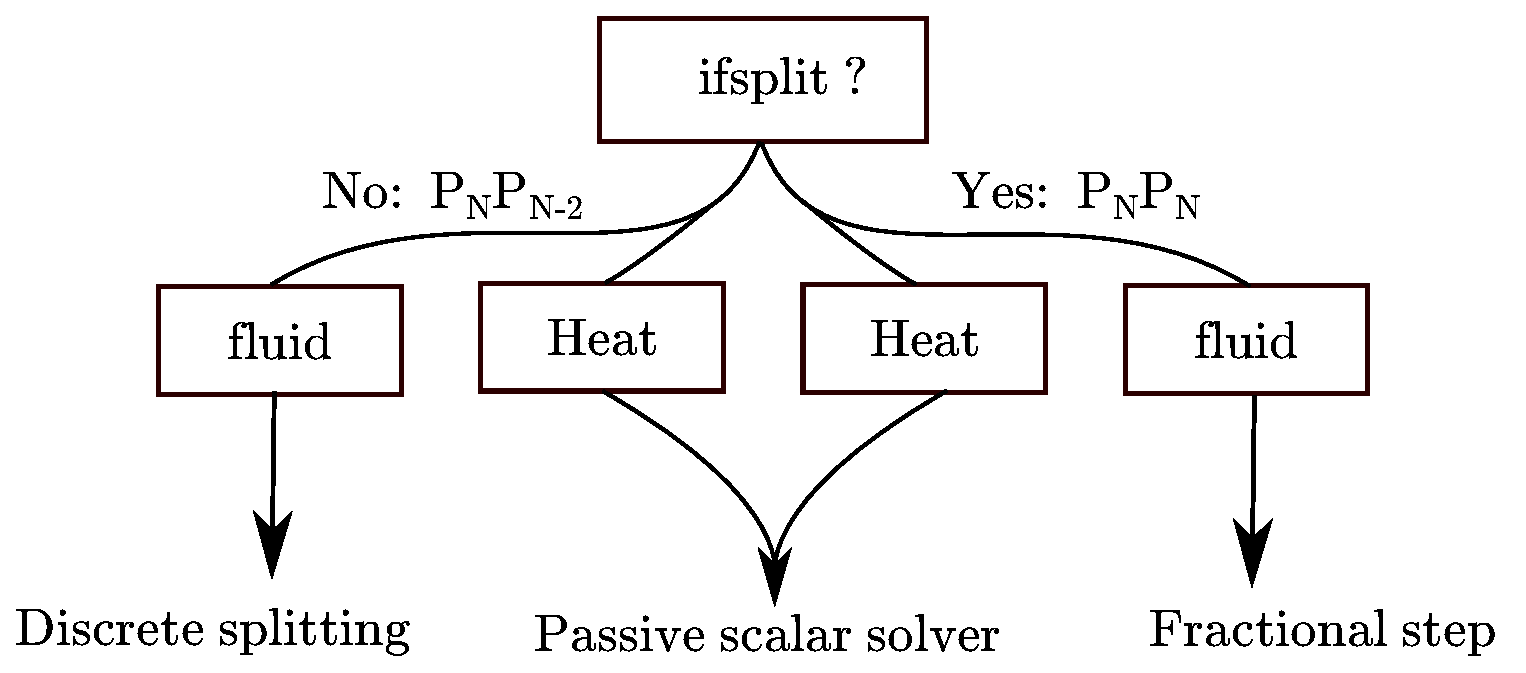
\includegraphics[width=0.8\textwidth]{Figures/Nek.pdf}
	\caption{Visualization of the steps in Nek5000.}
	\label{fig:files}
\end{figure}
%

The description of the routines corresponding to Pressure-correction and fractional step are found in 
\cref{prescorr} and~\ref{fracstep}. For further details regarding the 
implementation in Nek5000 it is referred to \cite{Fischer_hybridschwarz-multigrid}
and \cite{TomboulidesPnPn}. As mentioned before an important difference between these two implementations is the fact that the $P_NP_N$ 
implementation is based on an analytical splitting algorithm which introduces a non-vanishing error in the pressure along the boundaries of the 
domain while the $P_NP_{N-2}$ algorithm is a discrete splitting which does not explicitly force a wrong boundary condition.
It is however argumented in for instance~\cite{Guermond2006} that the discrete splitting also
introduces an erroneous boundary condition weakly.

%To best understand the work flow of Nek5000 the subroutine \verb|nek_advance| in \verb|drive1.f| should be examined.
%This routine includes all the steps in one iteration of the solver. The routine is adapted so that it is functional
%for a number of different problems and user defined settings. The most important boolean switches used in this routine are 
%described in the list below 
%
%\begin{itemize}
    %\item ifsplit - whether the $\mathbb{P}_N-\mathbb{P}_N$ or the $\mathbb{P}_N-\mathbb{P}_{N-2}$ is to be used.
    %\item iftrans - transient or steady flow.
    %\item ifheat - solving for heat.
    %\item ifnav - natural convection for the scalar fields (Boolean array)
    %\item param(103) - activation of filtering.
%\end{itemize}
%%
%further the routines of interests are \verb|fluid| and \verb|heat|, the solvers for N-S equations and passive scalars respectively.
%Both subroutines are found in \verb|drive2.f|. The understanding of these solvers are best achieved by studying equation  \eref{eq:NS} 
%and \eref{eq:PS}. For the settings chosen in this thesis a fractional step procedure as described in 
%\cref{fracstep} is applied.

%\colorbox{yellow}{what are fluidp() and heatp( )? solve for pertubated field and then project onto div-free space ? }

%\colorbox{yellow}{Talk about how the preconditioners work in Nek?}

%
%\section{Incompressible N-S solvers in Nek}
%Nek5000 offer several implementations depending on the mathematical formulation wanted by the user.
%The most standard, and the algorithm applied in this thesis is the fractional step procedure 
%described in detail in \cref{description}.


%A Convection-Diffusion problem can be stated as 
%\begin{align}
    %M\frac{du}{dt} = Au-Cu+Mf
    %\label{eq:conv-diff}
%\end{align}
%% 
%Where $M$ and $A$ is the mass, and stiffness matrix, $f$ is the loading function and $C$ is 
%the matrix corresponding to the convective term. The non-linearity is represented in the 
%convective term since $C$ is dependent of $u$.
%The time-derivative is discretized by a Backward difference (BDFk) scheme using solutions 
%from the $k$ previous steps to extrapolate the current value. In order to gain stability 
%an implicit scheme is chosen and the resulting eguation is given as 
%%
%OIFS ???
%---------- CHECK MAKEF IN NAVIER1.F ----------------- 
%\begin{align}
    %\sum_{j=0}^{k}\frac{b_j}{\Delta t}Mu^{n-j+1} = Au^{n+1}-Cu^{n+1}+Mf^{n+1}
    %\label{eq:conv-diff2}
%\end{align}
%% 
%By extrapolating the convective term from the $k$ previously calculated steps the equation 
%simplifies to 
%%
%\begin{align}
   %\frac{b_0}{\Delta t}Mu^{n+1} \sum_{j=1}^{k}\frac{b_j}{\Delta t}Mu^{n-j+1} 
   %= Au^{n+1}-\sum_{j=1}^{k}a_jCu^{n-j+1}+Mf^{n+1}
    %\label{eq:conv-diff3}
%\end{align}
%% 
%and finally by moving all the explicit terms to the rhs the equation left to solve is given as 
%%
%\begin{align}
   %(\frac{b_0}{\Delta t}M-A)u^{n+1} 
   %= -\sum_{j=1}^{k}(\frac{b_j}{\Delta t}M-a_jC)u^{n-j+1}+Mf^{n+1}
    %\label{eq:conv-diff4}
%\end{align}
%% 
%Notice from Section~\ref{theory} that this is equivalent to the matrix formulation of 
%the Helmholtz equation.



\section{Nek5000 for complex geometries}
For complex curved geometries such as bent cylinders, spheres, ellipsoids etc.
the user has to be able to express these surfaces analytically and write a routine
in \verb|usrdat2| that projects the points of interest onto the surface.
Even for a simple shape such as a sphere some implementation has to be done and it 
demands that the user has knowledge to Fortran77 and the structure of Nek5000.

The necessary implementation consists of two steps 
%
\begin{enumerate}
    \item determine the faces that belong to the deformed surface
    \item project the predefined GLL-points onto the deformed surface
\end{enumerate}
%
This can be done without too much work for shapes with a known analytical 
expression such as a cylinder or a sphere, but for some general CAD geometry 
it is no way to perform this projection routine. This is a vulnerable point 
for a SEM solver since the elements generated by the mesh are relatively coarse.
Many Finite volume based solvers do not support curved elements simply because the 
complex geometries are resolved with a sufficiently high resolution and it 
is of no interest to approximate them any better. However for a spectral element
solver it is necessary to address this problem since spectral convergence 
for the approximated solution in $\mathbb{P}_N$ is not achievable 
if the geometry is only represented in $\mathbb{P}_{1}$ or $\mathbb{P}_{2}$.

As a part of this thesis two advancements have been made regarding complex geometries. 
The first part is a fully automatic procedure which projects any edge onto a circle. This is a
convenient method when working with cylinder geometries and other similar shapes. The second part
is an attempt to include general boundary surfaces by creating a semi-automatic procedure allowing 
the user to represent any geometry with polynomials of the same order as applied for the basis functions.
The algorithms are presented in \cref{implementation}. 
